\subsection{Approach for Deepfake Detection}

For deepfake detection, our approach combines the power of vision transformers with advanced techniques in computer vision. Vision transformers excel in capturing both global and local features within an image, making them suitable for identifying subtle inconsistencies introduced by deepfake manipulation.
\\
\\
Our approach involves the following steps:

\noindent\textbf{Dataset Collection:} We gather a diverse dataset comprising real and deepfake images. This dataset is crucial for training and evaluating our deepfake detection model.
\\

\noindent \textbf{Vision Transformer Architecture:} We chose the Vision Transformer (ViT) architecture due to its ability to process image patches and learn relationships between them using self-attention mechanisms. ViT has shown impressive results in various computer vision tasks, and we adapt it for deepfake detection.
\\

\noindent\textbf{Preprocessing:} We preprocess the dataset to extract image patches and resize them to a consistent input size. These patches retain essential information while reducing computational complexity. Additionally, we normalize pixel values to ensure consistent input for the model.
\\

\noindent\textbf{Training:} During training, our vision transformer learns to differentiate between real and manipulated images. We use a binary cross-entropy loss function to optimize the model's weights. The self-attention mechanism in the ViT helps the model focus on relevant patches and capture intricate patterns indicative of deepfake manipulation.
\\

\noindent\textbf{Evaluation:} We evaluate the model's performance using various metrics such as accuracy, precision, recall, and F1-score. These metrics provide insights into how effectively the model distinguishes between real and deepfake images.
\\
\newpage
\noindent\textbf{Vision Transformer Architecture:}

\noindent The Vision Transformer (ViT) architecture comprises the following components:
\\

\noindent \textit{Patch Embedding:} Input images are divided into non-overlapping patches. Each patch is linearly projected to obtain embeddings, which are then augmented with positional encodings to maintain spatial information.
\\
\begin{figure}[h]
    \centering
    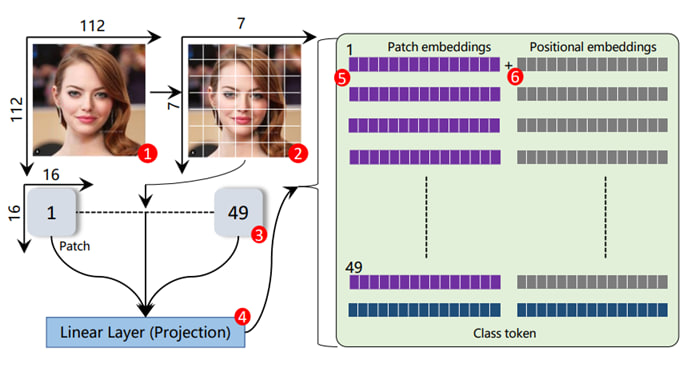
\includegraphics[width=6in]{img/patchembedding.jpg}
    \caption{Patch Embedding}
\end{figure}

\noindent \textit{Transformer Encoder:} The patch embeddings are fed into a stack of transformer encoder layers. Each layer consists of multi-head self-attention and feedforward neural networks. This enables the model to capture both local and global dependencies within the image.
\\
\begin{figure}[h]
    \centering
    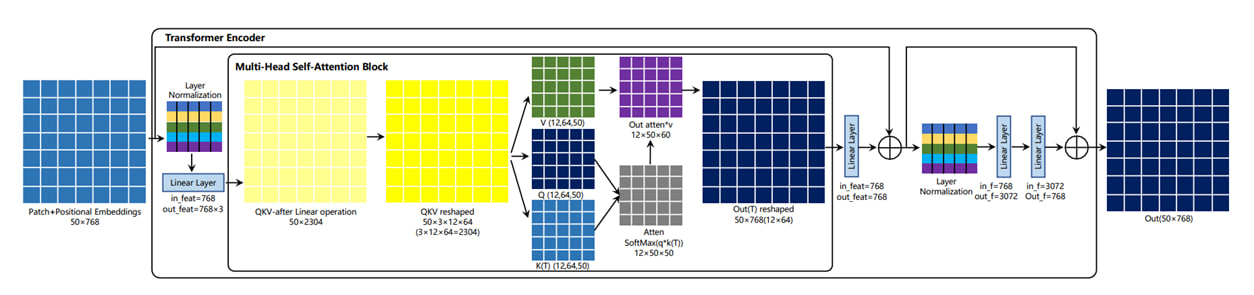
\includegraphics[width=6in]{img/encoderdetails.jpg}
    \caption{Transformer encoder}
\end{figure}
\newpage
\noindent \textit{Classification Head:} The final layer of the model serves as the classification head. It takes the transformed embeddings and predicts whether an image is real or manipulated.
\\

\begin{figure}[h]
    \centering
    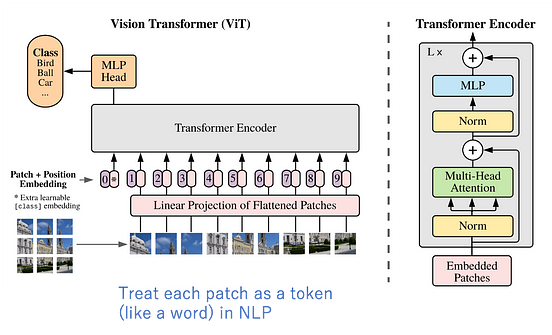
\includegraphics[width=6in]{img/visiontransformer.png}
    \caption{Vision Transformer Architecture}
\end{figure}

\newpage
\noindent \textbf{Steps:}
\vspace{0.2cm}

\noindent \textbf{Dataset Overview:}

\noindent Our dataset includes a diverse collection of real and deepfake images sourced from various public datasets and proprietary sources. It covers a wide range of scenarios, lighting conditions, and facial expressions to ensure the model's robustness. The dataset was meticulously curated to represent real-world variations and challenges that deepfake detection might encounter.

\noindent \textbf{Data Collection Process:}

\noindent Our dataset acquisition process involved the following steps:

\begin{enumerate}
    \item \textbf{Public Datasets:} We sourced a significant portion of our dataset from publicly available deepfake and real image datasets. These datasets were chosen for their variety and relevance to our detection task.

    \item \textbf{Proprietary Sources:} To further enhance the diversity of our dataset, we collaborated with proprietary sources that provided deepfake and real images. These sources helped us ensure a comprehensive representation of different contexts and manipulation techniques.

    \item \textbf{Video Conversion:} To include videos in our dataset, we first converted them into individual frames (images) to facilitate compatibility with the vision transformer architecture. This step involved extracting frames at a consistent frame rate from each video, resulting in a sequence of images for each video.

    \item \textbf{Frame Selection:} To avoid redundancy and maintain dataset balance, we carefully selected frames from videos to represent various stages of manipulation, expressions, poses, and lighting conditions.

    \item \textbf{Annotation and Labeling:} Each image was labeled as either "real" or "deepfake." Annotations were done manually to ensure accurate labeling for training and evaluation.
\end{enumerate}

\noindent \textbf{Preprocessing Techniques:}

\noindent Before training the model, we preprocess the dataset as follows:

\begin{enumerate}
    \item \textbf{Resize:} All images, whether sourced from videos or other datasets, were resized to a consistent resolution, such as 224x224 pixels. This resizing ensured a uniform input size for the vision transformer.

    \item \textbf{Augmentation:} To increase the dataset's diversity and improve the model's ability to generalize, we applied various data augmentation techniques. These techniques included random rotations, horizontal flips, brightness adjustments, and minor deformations.

    \item \textbf{Normalization:} Pixel values of the images were normalized to a specific range to ensure consistent input for the model during training and inference.
\end{enumerate}

\noindent By meticulously preprocessing the dataset, we enhanced the model's capacity to learn relevant features and intricate patterns required for accurate deepfake detection.

\noindent This comprehensive approach leverages the capabilities of vision transformers while customizing them to address the specific challenges associated with deepfake detection. By integrating diverse data sources and applying rigorous preprocessing steps, we developed a robust and efficient deepfake detection model that demonstrates impressive performance across various scenarios.



